\section{双向链表}

\begin{frame}\ft{定义(双向链表)}
双向链表:构成链表的每个结点设有两个指针域:
\begin{itemize}
\item[$\diamond$]
一个指向其直接前趋的指针域$prior$
\item[$\diamond$]
一个指向其直接后继的指针域$next$
\end{itemize}
这样形成的链表有两个不同方向不同的链,故称为双向链表。


\begin{itemize}
\item 和单链表类似,双向链表一般增加头指针,能使双向链表上的某些运算变得方便。
\item
将头结点和尾结点链接起来能构成循环链表,称之为双向循环链表。
\item
双向链表是为了克服单链表的单向性的缺陷而引入的。
\end{itemize}•
\end{frame}


\subsection{双向链表的结点及其类型定义}
\begin{frame}[fragile]\ft{\subsecname}
\begin{block}{双向链表结点的类型定义}
\begin{lstlisting}[language=C]
typedef struct DuLNode{
  ElemType data;
  struct DuLNode *prior, *next;
}DuLNode;
\end{lstlisting}
\end{block}

\begin{figure}
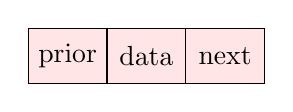
\begin{tikzpicture}
\def\x{1}
\def\y{0.7}
\def\r{0}
\foreach \c in {0,1,2}
\filldraw[fill=red!20,fill opacity=0.5] 
(\c+0.0*\x,\r+0.0*\y)rectangle(\c+1.0*\x,\r+\y);
\node[]at(0.5*\x,0.5*\y){prior};
\node[]at(1.5*\x,0.5*\y){data};
\node[]at(2.5*\x,0.5*\y){next};
\end{tikzpicture}
\caption{双向链表结点形式}
\end{figure}•
\end{frame}



\begin{frame}[fragile]\ft{\subsecname}
\begin{figure}
\centering
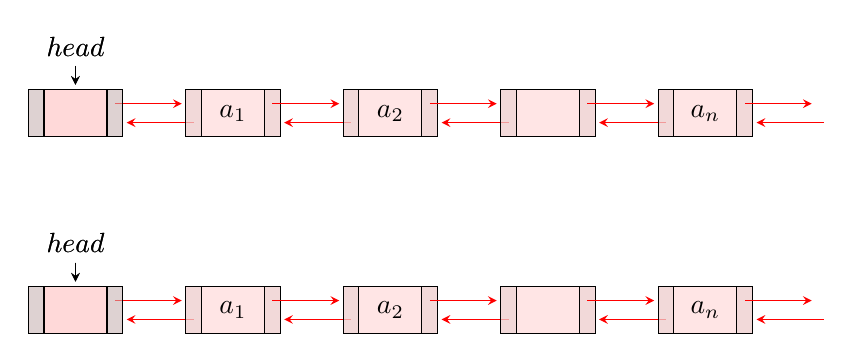
\begin{tikzpicture}[scale=1]
\def \x{1}
\def \y{0.6}

\foreach \c in {0,2.5}{
\ifthenelse{ 0 = \c}{
\foreach \r in {0,2,4,6,8}{
\ifthenelse{  6 = \r }{
\node[left] at (\r+\x,\c+0.5*\y) {$\cd$};
}{
\filldraw[fill=red!20,fill opacity=0.5](\r+0.2*\x,\c+0)rectangle(\r+1.0*\x,\c+\y);

\ifthenelse{  0 = \r }{
\filldraw[fill=black!20,fill opacity=0.5](\r+0.0*\x,\c+0)rectangle(\r+0.2*\x,\c+\y);  
}{
\filldraw[fill=red!20,fill opacity=0.5](\r+0.0*\x,\c+0)rectangle(\r+0.2*\x,\c+\y);
} 
\ifthenelse{  8 = \r }{
\filldraw[fill=black!20,fill opacity=0.5](\r+1.0*\x,\c+0)rectangle(\r+1.2*\x,\c+\y); 
}{
\filldraw[fill=red!20,fill opacity=0.5](\r+1.0*\x,\c+0)rectangle(\r+1.2*\x,\c+\y);
}
}
\ifthenelse{ 8 = \r}{
}{
\draw[<-,>=stealth,red] 
(\r+1.25*\x,\c+0.3*\y)--(\r+2.1*\x,\c+0.3*\y);
\draw[->,>=stealth,red] (\r+1.1*\x,\c+0.7*\y)
--(\r+1.95*\x,\c+0.7*\y);
}
}

\node[]at(2.6,\c+0.5*\y){$a_1$};
\node[]at(4.6,\c+0.5*\y){$a_2$}; 
\node[]at(8.6,\c+0.5*\y){$a_n$};
\draw[->,>=stealth] (0.6,\c+1.5*\y)node[above] {$head$} --(0.6,\c+1.1*\y);
}{
\foreach \r in {0}{
\filldraw[fill=black!20,fill opacity=0.5](\r+0.0*\x,\c+0)rectangle(\r+0.2*\x,\c+\y);  
\filldraw[fill=red!20,fill opacity=0.5](\r+0.2*\x,\c+0)rectangle(\r+1.0*\x,\c+\y); 
\filldraw[fill=black!20,fill opacity=0.5](\r+1.0*\x,\c+0)rectangle(\r+1.2*\x,\c+\y); 
\draw[->,>=stealth] (0.6,\c+1.5*\y)node[above] {$head$} --(0.6,\c+1.1*\y);
}
}
}

\end{tikzpicture}
\caption{带头结点的双向链表形式}
\end{figure}

\end{frame}

\begin{frame}[fragile]\ft{\subsecname}
双向链表结构具有对称性,设$p$指向双向链表中的某一个结点,则其对称性可描述为:
\begin{lstlisting}[frame=none]
(p->prior)->next=p=(p->next)->prior;
\end{lstlisting}
\end{frame}


\subsection{双向链表的基本操作}
\begin{frame}\ft{双向链表的插入}
将值为$e$的结点插入双向链表中,插入前后链表的变化如图:

\begin{figure}
\centering
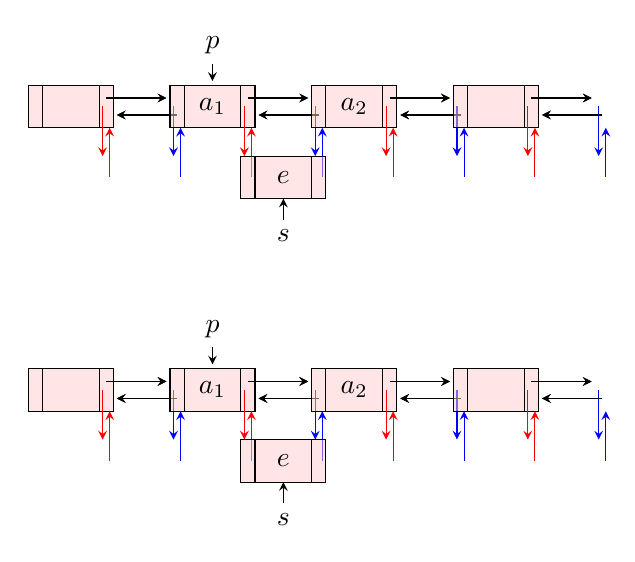
\begin{tikzpicture}[scale=0.9]
\def \x{1}
\def \y{0.6}

\foreach \c in {0,4}{
\foreach \r in {0,2,4,6}{
\ifthenelse{  0 = \r \OR 6 = \r}{
\node[left] at (\r+\x,\c+0.5*\y) {$\cd$};
}{
\filldraw[fill=red!20,fill opacity=0.5](\r+0.2*\x,\c+0)rectangle(\r+1.0*\x,\c+\y);
\filldraw[fill=red!20,fill opacity=0.5](\r+0.0*\x,\c+0)rectangle(\r+0.2*\x,\c+\y);
\filldraw[fill=red!20,fill opacity=0.5](\r+1.0*\x,\c+0)rectangle(\r+1.2*\x,\c+\y);
}

\ifthenelse{ 6 = \r \OR 2 = \r}{

\ifthenelse{ 2 = \r \AND \c = 4}
{
\draw[<-,>=stealth] 
(\r+1.25*\x,\c+0.3*\y)--(\r+2.1*\x,\c+0.3*\y);
\draw[->,>=stealth] (\r+1.1*\x,\c+0.7*\y)
--(\r+1.95*\x,\c+0.7*\y);
}{}

\ifthenelse{ 2 = \r \AND \c = 0}
{
\draw[->,>=stealth,red] 
(\r+1.05*\x,\c+0.5*\y)--(\r+1.05*\x,\c-1+\y);
\draw[<-,>=stealth,red] 
(\r+1.15*\x,\c)--(\r+1.15*\x,\c-1+0.5*\y);

\draw[->,>=stealth,blue] 
(\r+2.05*\x,\c+0.5*\y)--(\r+2.05*\x,\c-1+\y);
\draw[<-,>=stealth,blue] 
(\r+2.15*\x,\c)--(\r+2.15*\x,\c-1+0.5*\y);
}{}

}{
\draw[<-,>=stealth] 
(\r+1.25*\x,\c+0.3*\y)--(\r+2.1*\x,\c+0.3*\y);
\draw[->,>=stealth] (\r+1.1*\x,\c+0.7*\y)
--(\r+1.95*\x,\c+0.7*\y);
}
}

\node[]at(2.6,\c+0.5*\y){$a_1$};
\node[]at(4.6,\c+0.5*\y){$a_2$}; 
\draw[->,>=stealth] (2.6,\c+1.5*\y)node[above] {$p$} --(2.6,\c+1.1*\y);


\def\r{3}
\filldraw[fill=red!20,fill opacity=0.5](\r+0.2*\x,\c-1)rectangle(\r+1.0*\x,\c-1+\y);
\filldraw[fill=red!20,fill opacity=0.5](\r+0.0*\x,\c-1)rectangle(\r+0.2*\x,\c-1+\y);
\filldraw[fill=red!20,fill opacity=0.5](\r+1.0*\x,\c-1)rectangle(\r+1.2*\x,\c-1+\y);
\node[]at(\r+0.6*\x,\c-1+0.5*\y){$e$}; 
\draw[->,>=stealth] (\r+0.6*\x,\c-1-0.5*\y)node[below] {$s$} --(\r+0.6*\x,\c-1);

}

\end{tikzpicture}
\caption{双向链表的插入}
\end{figure}

\end{frame}


\begin{frame}[fragile]\ft{双向链表的插入}
\begin{itemize}
\item[(1)] 插入时仅仅指出直接前驱结点,钩链时必须注意先后次序“先右后左”。
\begin{lstlisting}[frame=none]
s=(DuLNode *)malloc(sizeof(DuLNode));
s->data=e;
s->next=p->next;
p->next->prior=s;
p->next=s;
s->prior=p;
\end{lstlisting}

\end{itemize}•

\end{frame}


\begin{frame}[fragile]\ft{双向链表的插入}
\begin{itemize}
\item[(2)] 插入时同时指出直接前驱结点$p$和直接后继结点$q$,钩链时无需注意先后次序。
\begin{lstlisting}[frame=none]
s=(DuLNode *)malloc(sizeof(DuLNode));
s->data=e;
p->next=s; s->next=q;
s->prior=p; q->prior=s;
\end{lstlisting}

\end{itemize}•

\end{frame}


\begin{frame}[fragile]\ft{双向链表的删除}
设要删除的结点为$p$,删除时可以不引入新的辅助变量,可以直接先断链,再释放结点。
\begin{lstlisting}[frame=none]
p->prior->next=p->next;
p->next->prior=p->prior;
free(p);
\end{lstlisting}
\pause

\begin{block}{注意}
与单链表的插入和删除操作不同的是,在双向链表中插入和删除必须同时修改两个方向上的指针域的指向。
\end{block}

\end{frame}